\section{Cuarta pregunta de investigación}
\label{sec:RQ4}

\noindent\fbox{%
\parbox{\dimexpr\textwidth-2\fboxsep-2\fboxrule\relax}{%
\textbf{RQ4} ¿Cómo influyen los algoritmos de balanceo de clases ROS, RUS y SMOTE en los resultados de los clasificadores?%
}%
}
\vspace{12pt}

\subsection{Desbalance de BugHunter}

La Tabla \ref{table:count_bug_nobug} muestra el número de instancias con error (\textit{bug}) y sin error por proyecto y nivel. En la mayoría de los proyectos predominan las instancias sin error, aunque la proporción varía considerablemente entre proyectos y niveles.

% Please add the following required packages to your document preamble:
% \usepackage{graphicx}
\begin{table}[H]
\captionsetup{labelsep=period, labelfont=bf}
\caption{\label{table:count_bug_nobug} Resumen de desequilibrio por nivel}
\centering
\resizebox{\textwidth}{!}{%
\begin{tabular}{lllllll}
\toprule
                               & \multicolumn{2}{c}{Método} & \multicolumn{2}{c}{Clase} & \multicolumn{2}{c}{Archivo} \\
                               \midrule
Proyecto                        & Bug       & Sin bug    & Bug      & Sin bug    & Bug      & Sin bug   \\
\midrule
oryx                           & 100       & 756            & 81       & 565            & 80       & 528           \\
antlr4                         & 132       & 768            & 132      & 230            & 156      & 223           \\
BroadleafCommerce              & 1337      & 3996           & 1569     & 1672           & 1733     & 1828          \\
mct                            & 26        & 81             & 21       & 51             & 15       & 43            \\
junit                          & 112       & 400            & 112      & 226            & 96       & 107           \\
netty                          & 3620      & 9923           & 2618     & 3973           & 2178     & 2947          \\
ceylon-ide-eclipse             & 660       & 1731           & 520      & 957            & 417      & 747           \\
titan                          & 287       & 736            & 195      & 311            & 199      & 287           \\
all                            & 58810     & 100268         & 41087    & 43475          & 35507    & 34581         \\
elasticsearch                  & 19784     & 31746          & 15769    & 15875          & 13068    & 12052         \\
mcMMO                          & 503       & 865            & 357      & 511            & 369      & 511           \\
orientdb                       & 4465      & 8732           & 2153     & 2617           & 2107     & 2341          \\
neo4j                          & 3175      & 6523           & 2068     & 2601           & 1824     & 2120          \\
hazelcast                      & 23830     & 32617          & 14926    & 13259          & 12881    & 10472         \\
MapDB                          & 644       & 1140           & 487      & 522            & 311      & 277           \\
Android-Universal-Image-Loader & 135       & 254            & 79       & 105            & 73       & 98        \\
\bottomrule
\end{tabular}%
}

\end{table}

La Tabla \ref{tab:desbalance} resume esta distribución tras binarizar el atributo \textit{Number of Bugs}. El desequilibrio de BugHunter es moderado si se compara con los conjuntos clásicos de PFS ---como NASA o PROMISE, donde la clase con error suele representar menos del 10\,\% de las instancias \cite{8494821}---: la mediana de instancias \textit{bug} entre los 15 proyectos es del 28,1\,\% a nivel de método, 41,1\,\% a nivel de clase y 42,7\,\% a nivel de archivo, y en tres proyectos (\textit{hazelcast}, \textit{MapDB} y \textit{elasticsearch}) la clase \textit{bug} llega a ser mayoritaria a nivel de archivo. Esta característica es consecuencia directa del diseño de BugHunter, que solo incluye elementos de código efectivamente afectados por errores. El caso más desequilibrado es \textit{oryx} (razón no-bug:bug de 7,6:1 a nivel de método), lo que debe tenerse presente al interpretar su desempeño, el más alto del estudio.

\begin{table}[H]
\centering
\caption{Proporción de instancias con error (\textit{bug}) por nivel de granularidad, sobre los 15 proyectos individuales}
\label{tab:desbalance}
\resizebox{\textwidth}{!}{%
\begin{tabular}{lccccc}
\toprule
Nivel & Mediana & Mín. (proyecto) & Máx. (proyecto) & ``All'' & Razón mediana \\
      & \% bug  &                 &                 & \% bug  & no-bug:bug \\
\midrule
Método  & 28,1 & 11,7 (\textit{oryx}) & 42,2 (\textit{hazelcast}) & 37,0 & 2,6:1 \\
Clase   & 41,1 & 12,5 (\textit{oryx}) & 53,0 (\textit{hazelcast}) & 48,6 & 1,4:1 \\
Archivo & 42,7 & 13,2 (\textit{oryx}) & 55,2 (\textit{hazelcast}) & 50,7 & 1,3:1 \\
\bottomrule
\end{tabular}}
\end{table}

\subsection{Efecto del balanceo sobre el \textit{F-measure} ponderado}

La Tabla \ref{tab:balance} resume el \textit{F-measure} promedio de las 13.916 ejecuciones agrupadas por técnica de balanceo, comparando el conjunto de entrenamiento original con su versión balanceada (el conjunto de prueba nunca se balancea). Con las tres técnicas, balancear el conjunto de entrenamiento no mejoró el \textit{F-measure} promedio respecto a entrenar con la distribución original. El efecto fue más marcado en RUS, cuya eliminación de instancias de la clase mayoritaria redujo la información disponible para el entrenamiento. Las desviaciones estándar fueron similares entre ambas condiciones (0,108 sin balancear; 0,104, 0,082 y 0,105 balanceando con ROS, RUS y SMOTE, respectivamente).

\begin{table}[H]
\centering
\caption{\textit{F-measure} promedio según técnica de balanceo (13.916 ejecuciones)}
\label{tab:balance}
\begin{tabular}{lccc}
\toprule
Técnica & Sin balancear & Balanceado & $\Delta$ \\
\midrule
ROS   & 0,555 & 0,548 & $-0{,}007$ \\
RUS   & 0,555 & 0,524 & $-0{,}031$ \\
SMOTE & 0,555 & 0,548 & $-0{,}007$ \\
\bottomrule
\end{tabular}
\end{table}

\begin{figure}[H]
    \centering
    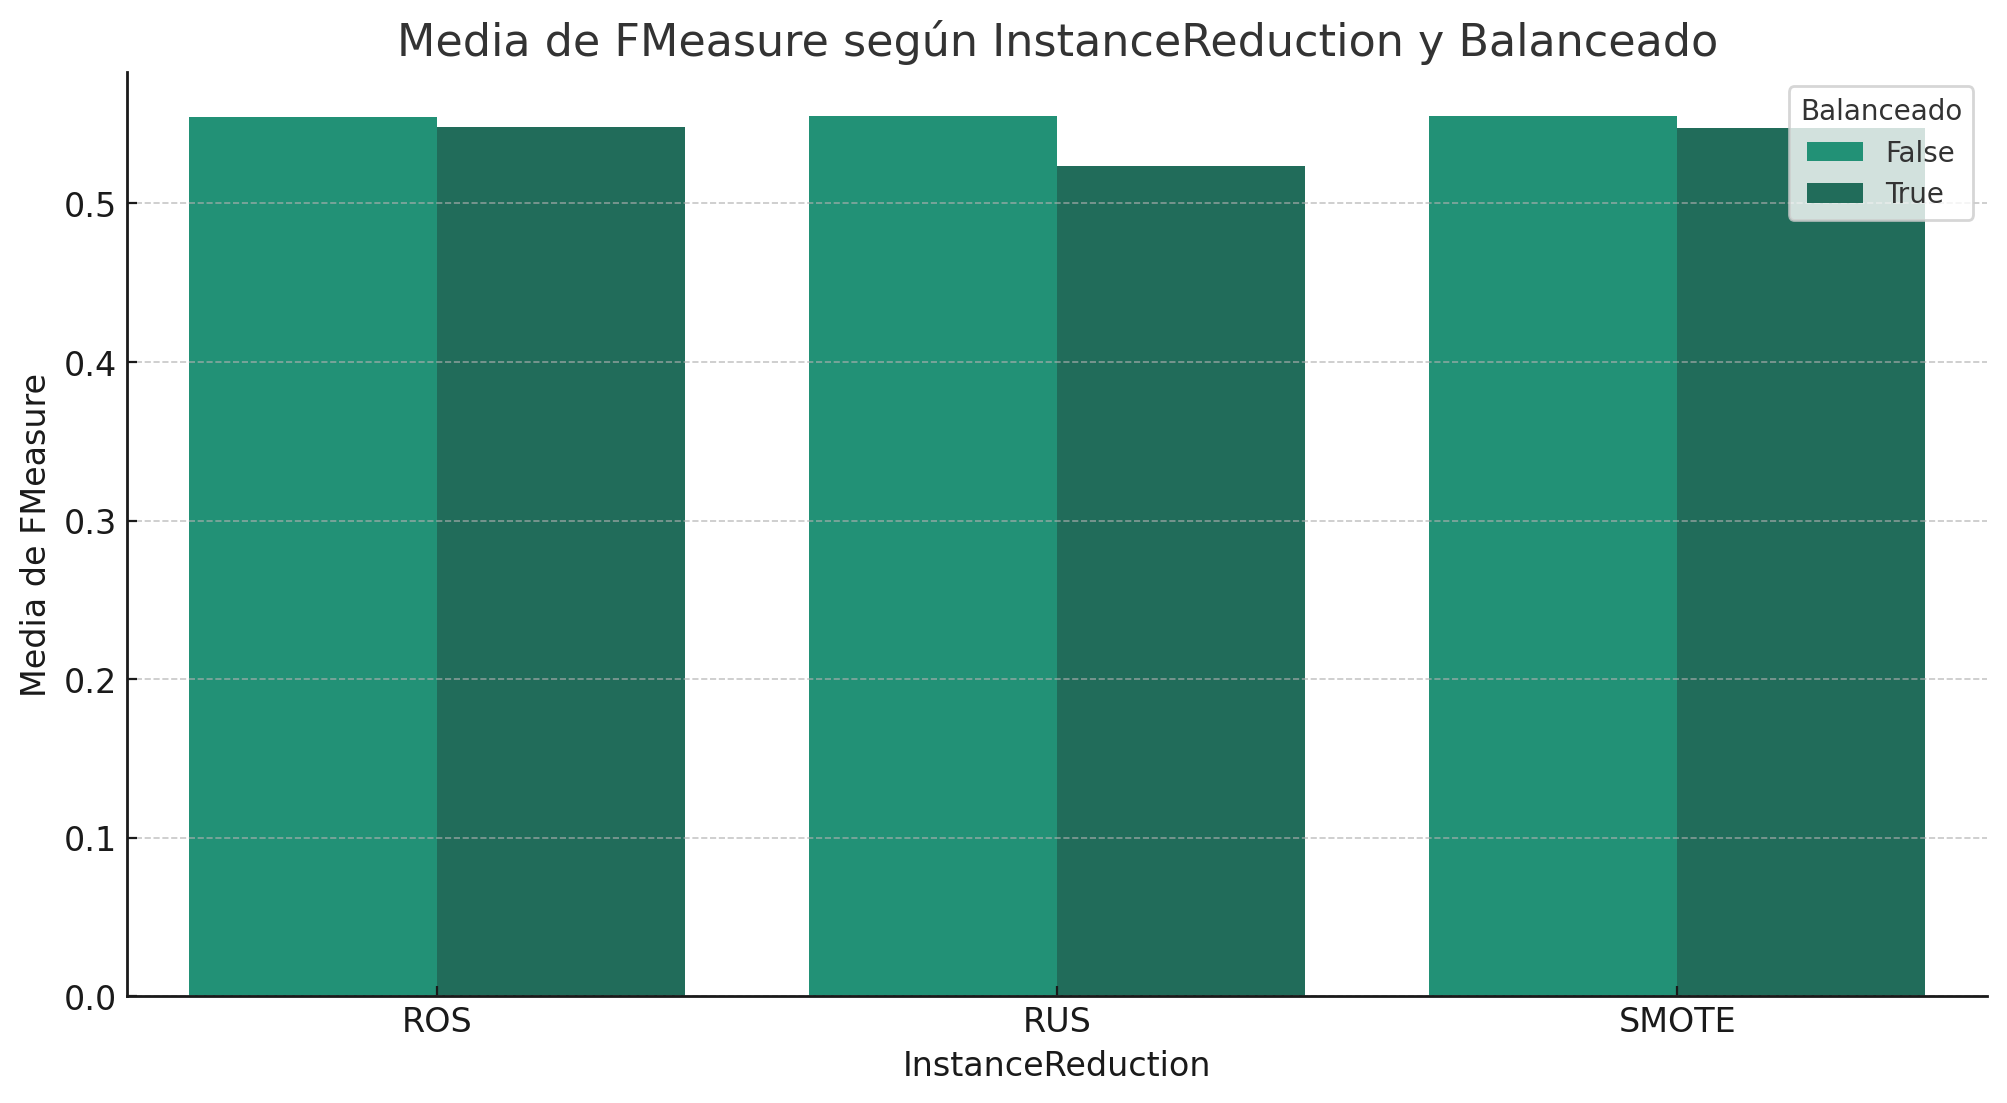
\includegraphics[width=150mm, height=120mm,]{chapters/chapter3/Sections/Research Questions/sections/RQ4/img/InstancereductionBalanceado.png}
     \setstretch{1} %Interlineado 1
	\captionsetup{labelsep=period, labelfont=bf}
    \caption{\textit{F-measure} medio según algoritmo de balanceo y condición de balanceo del entrenamiento}
    \label{fig:ROSRUSSMOTE}
\end{figure}

Para contrastar formalmente esta observación se aplicó una prueba de Wilcoxon de rangos con signo \cite{wilcoxon1945}, pareada por conjunto de datos, sobre el mejor \textit{F-measure} balanceado frente al mejor sin balancear de cada uno de los 16 conjuntos por nivel, complementada con el tamaño de efecto $\delta$ de Cliff \cite{cliff1993}. A nivel de método la diferencia resultó estadísticamente significativa a favor de la versión sin balancear ($p = 0{,}012$), aunque con un tamaño de efecto insignificante ($\delta = 0{,}07$); a nivel de clase ($p = 0{,}48$) y de archivo ($p = 0{,}86$) no se detectaron diferencias significativas, y al agrupar los tres niveles el resultado quedó en el límite de la significancia ($p = 0{,}052$). En los cuatro casos el tamaño de efecto fue insignificante ($|\delta| < 0{,}15$).

\subsection{Efecto del balanceo sobre la clase minoritaria}

Estas cifras deben interpretarse con cautela. Las medias de la Tabla \ref{tab:balance} se analizaron de forma descriptiva sobre todas las ejecuciones, mientras que la prueba estadística se aplicó a la mejor configuración por proyecto, sujeta a un sesgo de selección optimista. Además, el \textit{F-measure} agregado pondera ambas clases por su frecuencia, de modo que la contribución de la clase de interés práctico (\textit{bug}) queda diluida. Este efecto está acotado por el desequilibrio moderado de BugHunter (Tabla \ref{tab:desbalance}), pero no desaparece: la línea base del conjunto ``All'' a nivel de método (Tabla \ref{tab:porclase}) muestra que un \textit{F-measure} ponderado de 0,565 convive con un \textit{F-measure} de 0,356 para la clase \textit{bug} y un MCC cercano a cero.

Dos fuentes de evidencia permiten ir más allá de la métrica agregada. La primera son las matrices de confusión que Weka entrega para las mejores configuraciones a nivel de método (Tabla \ref{table:weka_method_smote_b}), a partir de las cuales se calculan el \textit{F-measure} de la clase \textit{bug} y el MCC (Sección \ref{sec:validacion_flujos}). Sobre los 16 conjuntos, entrenar con SMOTE reduce la mediana del \textit{F-measure} ponderado de 0,600 a 0,581, pero eleva la mediana del \textit{F-measure} de la clase \textit{bug} de 0,280 a 0,334; en MCC, en cambio, la diferencia es pequeña y de signo opuesto (0,070 frente a 0,056). Debe notarse que estas configuraciones fueron elegidas por su \textit{F-measure} ponderado y no por su desempeño en la clase minoritaria. La segunda fuente, más completa, es el análisis de sensibilidad (Sección \ref{sec:sensibilidad}), que almacena las métricas por clase para sus 28.440 ejecuciones y muestra que el balanceo mejora de forma consistente el \textit{F-measure} de la clase \textit{bug} y el MCC en los tres clasificadores evaluados, aun cuando el \textit{F-measure} ponderado apenas varía.

\subsection{¿Qué técnica de balanceo es más efectiva?}

La respuesta depende del objetivo. La Tabla \ref{tab:balanceo_tecnica} resume, sobre las ejecuciones del análisis de sensibilidad en los 15 proyectos individuales, la mediana de cada métrica según la técnica de balanceo. Con \textit{Random Forest} y XGBoost, RUS obtiene el mayor \textit{F-measure} de la clase \textit{bug} y el mejor MCC, pero también el menor \textit{F-measure} ponderado: al eliminar instancias de la clase mayoritaria, el modelo predice defectos con más frecuencia, lo que mejora su detección a costa de más falsos positivos. ROS y SMOTE ofrecen un compromiso intermedio, con mejoras más moderadas en la clase \textit{bug} y una pérdida menor en el agregado. Con la SVM lineal, las tres técnicas producen mejoras similares y grandes en la clase \textit{bug}, porque sin balanceo este clasificador casi no predice defectos. Por tanto, si el objetivo es detectar la mayor cantidad posible de código defectuoso, RUS es la técnica más efectiva; si se busca preservar el desempeño global, ROS o SMOTE son preferibles.

\begin{table}[H]
\centering
\caption{Mediana del desempeño por técnica de balanceo en el análisis de sensibilidad (15 proyectos individuales, todas las configuraciones)}
\label{tab:balanceo_tecnica}
\begin{tabular}{llccc}
\toprule
Clasificador & Balanceo & \textit{F-measure} ponderado & \textit{F-measure} bug & MCC \\
\midrule
RF   & Ninguno & 0,537 & 0,325 & $-0{,}015$ \\
RF   & ROS     & 0,529 & 0,356 & $-0{,}008$ \\
RF   & RUS     & 0,513 & 0,417 & 0,009 \\
RF   & SMOTE   & 0,532 & 0,343 & $-0{,}013$ \\
\midrule
XGB  & Ninguno & 0,540 & 0,318 & 0,003 \\
XGB  & ROS     & 0,537 & 0,367 & 0,001 \\
XGB  & RUS     & 0,524 & 0,427 & 0,027 \\
XGB  & SMOTE   & 0,542 & 0,346 & $-0{,}004$ \\
\midrule
SVM  & Ninguno & 0,551 & 0,171 & 0,038 \\
SVM  & ROS     & 0,562 & 0,423 & 0,086 \\
SVM  & RUS     & 0,558 & 0,426 & 0,081 \\
SVM  & SMOTE   & 0,565 & 0,425 & 0,087 \\
\bottomrule
\end{tabular}
\end{table}

Las medianas de MCC cercanas a cero reflejan que la tabla incluye todas las configuraciones de selección, también las peores; las mejoras sobre la mejor configuración de cada proyecto se presentan en la Tabla \ref{tab:sensibilidad}.

\noindent\fbox{%
\parbox{\dimexpr\textwidth-2\fboxsep-2\fboxrule\relax}{%
\textbf{Respuesta RQ4}
Balancear solo el conjunto de entrenamiento con ROS, RUS o SMOTE no mejora el \textit{F-measure} ponderado cuando el conjunto de prueba conserva la distribución real de clases; RUS lo empeora de forma más marcada ($-0{,}031$). La diferencia entre las mejores configuraciones con y sin balanceo tiene un tamaño de efecto insignificante ($|\delta| < 0{,}15$) en los tres niveles. Sin embargo, el balanceo sí desplaza el desempeño hacia la clase de interés práctico: aumenta el \textit{F-measure} de la clase \textit{bug} y, en el análisis de sensibilidad, también el MCC. La conclusión de RQ4 depende, por tanto, de la métrica de evaluación empleada. Entre las técnicas, RUS maximiza la detección de defectos y ROS y SMOTE preservan mejor el desempeño global.
}%
}
\vspace{12pt}
